\documentclass{article}
\usepackage[top=2.5cm, bottom=2cm, left=3cm, right=2cm]{geometry}
\usepackage[utf8]{inputenc}
\usepackage{amsthm}
%\usepackage[]{babel}
\usepackage{amssymb}
\usepackage{amsmath}
\usepackage{graphicx}
\usepackage{bm}
\usepackage{listings}
\usepackage{indentfirst}
%\usepackage{hyperref}

\newtheorem{theorem}{Theorem}[section]
\newtheorem{corollary}{Corollary}[theorem]
\newtheorem{lemma}[theorem]{Lemma}

\renewcommand\qedsymbol{$\blacksquare$}

\renewcommand{\contentsname}{\center{Sumário}}
%%%%%%%%%%%%%%%%%%%%%%%%%%%%%%%%%%%% Python Codes %%%%%%%%%%%%%%%%%%%%%%%%%%%%%%%%%%%%%%%%%%%%%%%%%%%%%%%%%%%%%%%%%%%%%%%%%%

% Default fixed font does not support bold face
\DeclareFixedFont{\ttb}{T1}{txtt}{bx}{n}{10} % for bold
\DeclareFixedFont{\ttm}{T1}{txtt}{m}{n}{10}  % for normal

% Custom colors
\usepackage{color}
\definecolor{deepblue}{rgb}{0,0,0.5}
\definecolor{deepred}{rgb}{0.6,0,0}
\definecolor{deepgreen}{rgb}{0,0.5,0}

% Python style for highlighting
\newcommand\pythonstyle{\lstset{
language=Python,
basicstyle=\ttm,
otherkeywords={self},             % Add keywords here
keywordstyle=\ttb\color{deepblue},
emph={MyClass,__init__},          % Custom highlighting
emphstyle=\ttb\color{deepred},    % Custom highlighting style
stringstyle=\color{deepgreen},
frame=tb,                         % Any extra options here
showstringspaces=false            % 
}}

% Python environment
\lstnewenvironment{python}[1][]
{
\pythonstyle
\lstset{#1}
}
{}

% Python for external files
\newcommand\pythonexternal[2][]{{
\pythonstyle
\lstinputlisting[#1]{#2}}}

% Python for inline
\newcommand\pythoninline[1]{{\pythonstyle\lstinline!#1!}}

%%%%%%%%%%%%%%%%%%%%%%%%%%%%%%%%%%%%%%%%%%%%%%%%%%%%%%%%%%%%%%%%%%%%%%%%%%%%%%%%%%%%%%%%%%%%%%%%%%%%%%%%%%%%%%%%%%%%%%%%%%%%

\begin{document}

\theoremstyle{definition}
\newtheorem{definition}{Definition}[section]

\begin{center}

FIS0610 - Física Computacional I

\vspace{1em}
{\Huge Uma Breve Introdução ao Python\footnote{Python 2.7.12}}

\vspace{1em}
Paulo Douglas Santos de Lima\\
\texttt{paulo.douglas.lima@dfte.ufrn.br}\\

\end{center}

\tableofcontents

\newpage

\section{Problema 1}
\pythonexternal{ex1.py}

\section{Problema 2}
\pythonexternal{ex2.py}
\section{Problema 3}
\pythonexternal{ex3.py}
\section{Problema 4}
\pythonexternal{ex4.py}
\pythonexternal{ex4a.py}
\begin{center}
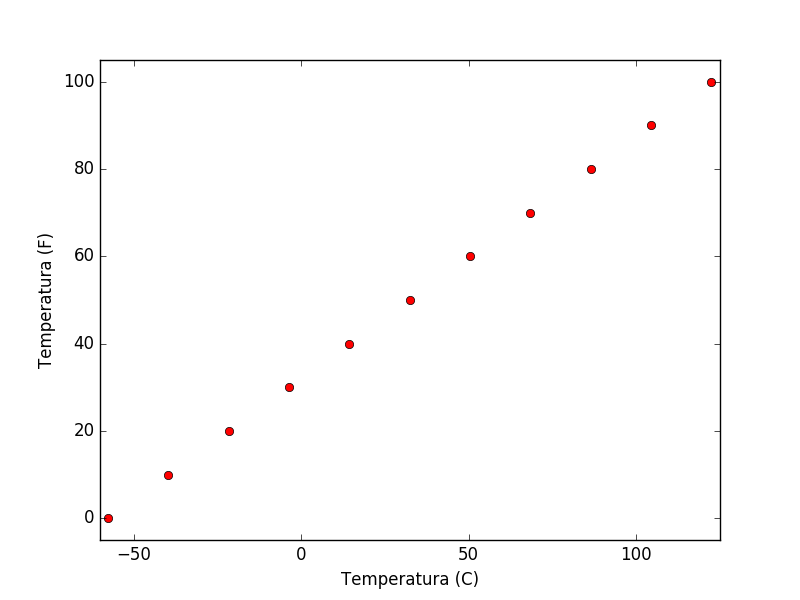
\includegraphics[scale=0.75]{ex4}
\end{center}
\section{Problema 5}
\pythonexternal{ex5.py}

\end{document}








\grid
